% First we choose the document class (can be book, report, article etc.)
\documentclass[11pt]{article}
\usepackage{amsmath}

\usepackage[table]{xcolor}
 
\usepackage{xcolor}
\usepackage{listings}

\lstdefinestyle{customc}{
  belowcaptionskip=1\baselineskip,
  breaklines=true,
  frame=L,
  xleftmargin=\parindent,
  language=C,
  showstringspaces=false,
  basicstyle=\footnotesize\ttfamily,
  keywordstyle=\bfseries\color{green!40!black},
  commentstyle=\ttfamily\color{purple!40!black},
  identifierstyle=\color{blue},
  stringstyle=\color{orange},
}
\lstset{escapechar=@,style=customc}

\usepackage{graphicx}

\author{Edward LaFemina \\
		\it{University of Maryland, Baltimore County}}
\title{Math 627 HW 3}
\date{\today}

\begin{document}
\maketitle
\tableofcontents

\pagebreak
\section{Problem 1}
I will be creating a series of standard matrix and vector functions for later use in an algorithm to estimate the largest eigenvalue of a square matrix. I will be verifying that these functions work individually, are accurate, and work on matrices and vectors distributed across multiple processes.

\subsection{Printing a Matrix}
The function written for this part must be able to print out the full contents of a matrix that is distributed across many processes. My function requires a pointer\(\texttt{l\_A}\) to that process's chunk of the matrix, the length of a row of the matrix\(\texttt{n}\) because it assumes A is square, the id of the process\(\texttt{id}\), and the number of processes\(\texttt{np}\). It then allocates enough memory for $ n^2 $ \texttt{double}s on process $ 0 $ to allow for assembling a full copy of the matrix. The function uses the \texttt{MPI\_Gather} function provided by MPI to get every process's chunk of A into the space allocated on process 0 in the right order. Because there are \texttt{np} processes and $ n $ columns of the matrix, each process holds $ l\_n = n / np $ columns of $ n $ \texttt{double}s, meaning each process had to send $ n*l\_n $ doubles to process $ 0 $. This was reflected in the call to \texttt{MPI\_Gather} in both the \texttt{send\_count} and \texttt{recv\_count} arguments. The function encodes a matrix A in the form:
$$
A_{n,n} =
\begin{pmatrix}
	a_{1,1} & a_{1,2} & \cdots & a_{1,n} \\
	a_{2,1} & a_{2,2} & \cdots & a_{2,n} \\
	\vdots  & \vdots  & \ddots & \vdots  \\
	a_{n,1} & a_{n,2} & \cdots & a_{n,n} 
\end{pmatrix}
$$
 to a single array in memory of the form:
$$
\begin{matrix} 
value |& a_{1,1} & a_{2,1} & \cdots & a_{n,1} & a_{1,2} & \cdots & a_{n,2} & \cdots & a_{n,n} \\
index |& 0       & 1       & \cdots & n-1       & n       & \cdots & 2*n - 1   & \cdots & n*n
\end{matrix}
$$
storing it only on process $ 0 $. To print the matrix in a human readable format, the function loops $ n $ times, printing the next element in the array each time. After $ n $ iterations, a newline character is printed. This repeats $ n $ times to account for all $ n $ rows.

To verify that the matrix prints as expected, I printed the matrix created by the \texttt{setup\_example} function written by Dr. Gobbert and supplied to me, in which each element $a_{i,j}=\frac{1}{i+j}$. Because this matrix is equal to its transpose, I altered the element in what should be the bottom left corner of the matrix to be $ 0 $, a value that does not appear anywhere else in the matrix. When printing, this value appeared in the bottom left corner of the matrix and all values for the other cells matched what I had computed them to be by hand for some small values of $n$.

\subsection{Dot Product}
The function written for this part must be able to compute the dot product of two column vectors of length $ n $ distributed over $ np $ processes and have the result available on all processes. To accomplish this, my function takes pointers to portions of both vectors, \texttt{l\_x} and \texttt{l\_y} which are of length $ l\_n = n / np $, the length\(\texttt{n}\) of the full vectors, the id of the process\(\texttt{id}\), and the number of processes\(\texttt{np}\). It then computes the product of the $i$-th element in each vector with the corresponding element in the other vector and adds that to a running total of the local dot product called \texttt{l\_sum}. To compute the dot product of the full vectors and make the result available on all processes, the function calls \texttt{MPI\_Allreduce} with the operation \texttt{MPI\_SUM} to indicate that all local \texttt{l\_sum} values shall be added together and then stored in every process's \texttt{dot\_product} variable which is returned by the function. Thus each process that calls this function will obtain the exact same result, which is the dot product of the global vectors \texttt{x} and \texttt{y} which have been distributed over all processes in \texttt{l\_x} and \texttt{l\_y} respectively.

I verified my function by computing the dot product between the even and odd vectors I created earlier and matching the returned answer to the answer I was able to compute with Matlab. In all cases my function gave the correct answer. To be sure that every process received the same value, I had every process create a message with the value of the dot product in it and sent the message to process $0$. I then had process $0$ print the message along with the \texttt{MPI\_SOURCE} value in the status struct created upon receipt of the message. In all tests the values were identical among all processes.

\subsection{Euclidean Vector Norm}
The function written for this part must compute the Euclidean Vector Norm of a vector \texttt{x} distributed amongst \texttt{np} processes and have the answer available to all processes. To compute this, my function took the square root of the dot product of \texttt{x} with itself using the \texttt{sqrt} function in the standard math library and returned it. Because the dot product is shared among all processes, the square root of that value is the same among all processes, therefore the value of the Euclidean Norm is the same on all processes.

To verify my function, I computed the Euclidean Norm of the odd vector I had created earlier using Matlab and used that result to verify the value my function returned. Because the dot product is distributed to all processes and I already verified this was the case, I knew the square root of that value would be the same among all processes and no further testing was needed.

\subsection{Matrix-Vector Product}
The function written for this part must compute the product $y=A*x$ where $A$ is an $n \times n$ square matrix and $x$ is a column vector of dimension $n$ and $y, A,$ and $x$ are distributed across \texttt{np} processes. To accomplish this, my function takes pointers to the locally held portion of A called \texttt{l\_A}, the locally held portion of x called \texttt{l\_x}, the length\(\texttt{n}\) of a column of A, the id of the process\(\texttt{id}\), and the number of processes\(\texttt{np}\). It also takes a pointer to a vector of length $ l\_n = n / np $ to store the final result in, and two pointers to \texttt{n} vectors to temporarily store copies of the full vector \texttt{y} as it is computed on several different processes.

For each of the \texttt{l\_n} columns referenced by \texttt{l\_A}, the function computes the product of the $j$-th element in the $i$-th column of \texttt{l\_A} with the $i$-th element of \texttt{l\_x} and adds that to a running total. The running total is stored as the $j$-th value of a temporary vector \texttt{temp\_y}. When this is complete, \texttt{temp\_y} has only partial sums of the dot product of each column of \texttt{A} with \texttt{x}. To complete \texttt{y}, my function calls \texttt{MPI\_Reduce} with the operation \texttt{MPI\_SUM} which stores the final resultant vector \texttt{y} in the second temporary storage vector. This is then distributed across all processes using \texttt{MPI\_Scatter} into the local vectors \texttt{l\_y}.

To verify this function for correctness, I computed the matrix-vector product of the matrix \texttt{A} created by the \texttt{setup\_example} function supplied and the vector of odd numbers created for earlier testing in Matlab and used that result to check the value given by my function. In all cases, the Matlab answer and my function's answer were the same, however the $15$th digit after the decimal place in the Matlab answer was occasionally $1$ higher than the corresponding digit in the answer returned by my function which I suspect is due to how Matlab handles rounding and not due to an inaccuracy in my function.
\pagebreak
\section{Problem 2}
The purpose of thise problem is to write a function that can compute the largest eigenvale and associated eigenvector of an $n \times n$ matrix $A$ within a given tolerance $tol$ using an iterative process called the Power Method of a matrix that is distributed over several processors. The Power Method starts with an initial guess of a column vector $x_{0}$ of $n$ elements. For our purposes, we set every element of $x_{0}$ equal to $\frac{1}{\sqrt{n}}$. The algorithm then performs the computation $x_{i+1}=A*x_{i}$, starting with $x_{1}=A*x_{0}$. It then computes the eigenvalue $\lambda_{i}$ from the computed $x_{i}$; my implementation uses the Rayleigh Quotient to compute 
$$\lambda_{i}=\frac{A*x_{i}}{x_{i}\cdot x_{i}}.$$
To determine if the approximation is close enough to the actual value of the eigenvalue, we test if 
$$\left|\frac{\lambda_{i}-\lambda_{i-1}}{\lambda_{i}}\right| < tol.$$ 
If it is not, the algorithm performs iterations until this condition is satisfied, or until a maximum number of iterations has been reached.

My implementation of the Power Method takes as input a pointer to the distributed column vector $l\_x$ to be used as the initial guess and the resulting eigenvector, $l\_y$ as a temporary column vector to be used in operations, a pointer to the distributed matrix $l\_A$, the tolerance $tol$, a max number of iterations to be completed $itmax$, the dimensions of the matrix and column vectors $n$, the id of the current process $id$, and the number of processes $np$. It also takes pointers to $lambda$ and $err$ to store the approximated eigenvalue and associated error. By looking at the Matlab code given to me by Dr. Gobbert, I was able to replicate most of the statements into my function.

My function starts by computing $y=A*x$ using the maxtrix vector multiplication function I created in Problem 1. I set $err=1+tol$ to ensure my code will perform at least one iteration of the Power Method, just as the Matlab code does. I set $\lambda_{0}=0$ as the Matlab code does in order to provide a starting point for my approximation. For the condition of my iteration, I verify that the error is greater than the tolerance and the maximum number of iterations has not been met before continuing the Power Method. To compute the next iteration of the approximation, I first save the most recent approximation in \texttt{l\_x}, then I use the matrix vector multiplication function I created earlier. I then compute the eigenvalue from the approximation with the Rayleigh quotient. It then computes the error from the last approximation using the formula mentioned above. If the maximum number of iterations is reached, a warning message is printed and the function exits, storing the most recent approximation in $ l\_x $.

Running my code with several values of \texttt{n}, the length of a column of \texttt{A}, resulted reoughly increasing residuals, indicating the approximation of the eigenvector was getting further from the actual eigenvector. I say roughly increasing because when running with $n=4$ the residual was $1.3759444812616986\times 10^{-7}$, at $n=4096$ it was $1.1144453159295350\times 10^{-6}$ which is about $10$ times larger, however at $n=8192$, the residual dropped down to $7.4383595482650898\times 10^{-7}$ which is larger than the residual for $n=4$ but smaller than that of $n=4096$. The residual continues to increase until at least $n=32768$.
\pagebreak

\section{Problem 3}
In order to time my code efficiently, I have conducted an analysis of memory usage to determine the largest value of $n$ I can use as a dimension of my matrix to avoid running out of memory. I will base my judgement of the maximum value of $n$ I can test with on how much memory an $n \times n$ matrix consumes when run on only one process. The largest variable in my program is \texttt{l\_A} by far, having $n^2$ elements of type \texttt{double}. A \texttt{double} takes up $8$ bytes of space, meaning \texttt{A} takes up $8n^2$ bytes. The following table displays the approximate memory use of my program for different values of $n$:

Because I will be running my program on the hcpf2013 nodes, each with $64$ GB of memory, I will only run tests that I project to use less than $64$ GB of memory.
\begin{center}
\begin{tabular}{ |c|c| } 
\hline
n & size in GB \\
\hline
$4 $& $1.1920 \times 10^{-7} $\\ 
$32$ & $7.6920 \times 10^{-6} $\\
$1024$ & $7.8125 \times 10^{-3} $\\
$2048$ & $3.125 \times 10^{-2} $\\
$4096$ & $1.25 \times 10^{-1} $\\
$8192$ & $ .5 $\\
$16384$ & $ 2 $\\
$32768$ & $  8 $\\
$65536$ & $ 32$\\
$131072$ & $ 128 $\\
\hline
\end{tabular}
\end{center}
Because values of $n<1024$ make exceptionally small matrices, I suspect my Power Method approximation will take $<1$ second and I will not be reporting on times for such tests. INstead, I will report on times needed to perform the approximation at the values of $n$ listed in the table $\geq 1024$. I will run the tests on hcpf2013 nodes with $8$ processes per node, except for $p = 1$ for which I will use $1$ process per node, $p = 2$ for which I will use $2$ processes per node, $p = 4$ for which I will use $4$ processes per node, and $p = 1024$ for which I will use $16$ processes per node. I have chosen this distribution of tasks per node because findings in HPCF-2015-6 indicate that using $8$ tasks per processor is best when using memory bound code, however we must use $16$ tasks for the last value of $p$ to fit $1024$ processes on $64$ nodes. I set the maximum number of iterations to $50$ because in all tests so far I have not reached any more than $40$ and the tolerance to $1 \times 10^{-12}$ for the same reason. The table below documents my results:


\begin{table}
\makebox[\linewidth]{
\begin{tabular}{ |c|c|c|c|c|c|c|c|c|  }
\hline
\multicolumn{9}{|c|}{Observed Wall Time in seconds}\\
\hline
$N     $&$ p=1   $&$ p=2   $&$ p=4   $&$ p=8   $&$ p=16  $&$ p=32  $&$ p=64  $&$ p=128 $\\
\hline
$1024  $&$ 0.02  $&$ 0.01  $&$ <0.00 $&$ <0.00 $&$ <0.00 $&$ <0.00 $&$ <0.00 $&$ <0.00 $\\
$2048  $&$ 0.01  $&$ 0.04  $&$ 0.02  $&$ 0.01  $&$ 0.01  $&$ <0.00 $&$ <0.00 $&$ 0.01  $\\
$4096  $&$ 0.04  $&$ 0.02  $&$ 0.13  $&$ 0.06  $&$ 0.04  $&$ 0.02  $&$ 0.01  $&$ 0.01  $\\
$8192  $&$ 1.98  $&$ 1.03  $&$ 0.54  $&$ 0.29  $&$ 0.15  $&$ 0.08  $&$ 0.05  $&$ 0.05  $\\
$16384 $&$ 8.51  $&$ 4.32  $&$ 2.28  $&$ 1.28  $&$ 0.64  $&$ 0.33  $&$ 0.18  $&$ 0.13  $\\
$32768 $&$ 37.36 $&$ 18.78 $&$ 9.98  $&$ 5.48  $&$ 2.73  $&$ 1.40  $&$ 0.75  $&$ 0.46  $\\
\hline
\hline
\multicolumn{9}{|c|}{Observed Speedup $S_p$}\\
\hline
$N     $&$ p=1   $&$ p=2   $&$ p=4   $&$ p=8   $&$ p=16  $&$ p=32  $&$ p=64  $&$ p=128 $\\
\hline
$1024  $&$ 1.00  $&$ 1.85  $&$ 3.29  $&$ 5.83  $&$ 3.96  $&$ 4.07  $&$ 1.32  $&$ 2.43  $\\
$2048  $&$ 1.00  $&$ 2.19  $&$ 3.94  $&$ 7.51  $&$ 8.97  $&$ 12.17 $&$ 10.62 $&$ 9.94  $\\
$4096  $&$ 1.00  $&$ 1.95  $&$ 3.35  $&$ 6.51  $&$ 10.96 $&$ 19.24 $&$ 27.66 $&$ 28.84 $\\
$8192  $&$ 1.00  $&$ 1.92  $&$ 3.65  $&$ 6.63  $&$ 12.58 $&$ 22.49 $&$ 38.20 $&$ 37.49 $\\
$16384 $&$ 1.00  $&$ 1.96  $&$ 3.72  $&$ 6.64  $&$ 13.13 $&$ 25.09 $&$ 45.02 $&$ 63.60 $\\
$32768 $&$ 1.00  $&$ 1.98  $&$ 3.74  $&$ 6.81  $&$ 13.66 $&$ 29.66 $&$ 49.22 $&$ 80.82 $\\
\hline
\hline
\multicolumn{9}{|c|}{Observed Efficiency $E_p$}\\
\hline
$N     $&$ p=1   $&$ p=2   $&$ p=4   $&$ p=8   $&$ p=16  $&$ p=32  $&$ p=64  $&$ p=128 $\\
\hline
$1024  $&$ 1.00  $&$ 0.925  $&$ 0.8225  $&$ 0.7287  $&$ 0.2475  $&$ 0.1271  $&$ 0.0206  $&$ 0.0189  $\\
$2048  $&$ 1.00  $&$ 1.095  $&$ 0.9850  $&$ 0.9387  $&$ 0.5606  $&$ 0.3803 $&$ 0.1659 $&$ 0.0776  $\\
$4096  $&$ 1.00  $&$ 0.975  $&$ 0.8375  $&$ 0.8137  $&$ 0.6850 $&$ 0.6012 $&$ 0.4321 $&$ 0.2253 $\\
$8192  $&$ 1.00  $&$ 0.960  $&$ 0.9125  $&$ 0.8287  $&$ 0.7862 $&$ 0.7028 $&$ 0.5968 $&$ 0.2928 $\\
$16384 $&$ 1.00  $&$ 0.980  $&$ 0.9300  $&$ 0.8300  $&$ 0.8206 $&$ 0.7840 $&$ 0.7034 $&$ 0.4968 $\\
$32768 $&$ 1.00  $&$ 0.990  $&$ 0.9350  $&$ 0.8512  $&$ 0.8537 $&$ 0.9268 $&$ 0.7690 $&$ 0.6314 $\\
\hline
\hline
\end{tabular}
}
\end{table}
\begin{figure}
\caption{The Observed Speedup with various numbers of parallel processors as well as an ideal line.}
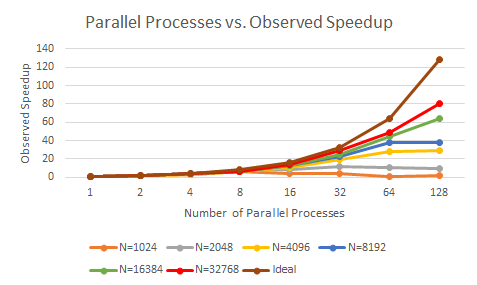
\includegraphics{speedup.png}
\end{figure}
\begin{figure}
\caption{The Observed Efficiency with various numbers of parallel processes as well as an ideal line.}
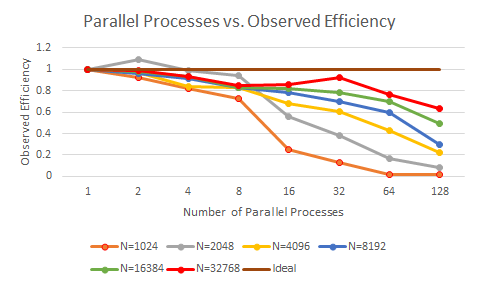
\includegraphics{efficiency.png}
\end{figure}
When running tests, I noticed some tasks were not running because the max CPU limit had been reached on the current QoS. I then switched from normal to short to allow my program to use all $64$ hpcf2013 CPUs in the batch partition. This solved that problem, however I also recieved the following error when running on $32$ and $64$ nodes: \texttt{MPI startup(): ofa fabric is not available and fallback fabric is not enabled}. This seems to be related to the Connect-IB HCA on the InfiniBand adapter. I am unsure of how to resolve the issue, but my first instinct is to retry the test at a later time. Upon retrial, I received the same error messages. Tests that would have run with $n=65536$ errored out in some cases. From my memory usage estimation, \texttt{A} should use $32$ GB on a node at any one time. However when the matrix \texttt{A} is distributed over only $1$ node, my program is unable to allocate enough memory and cannot complete the approximation.

Regarding times, it is clear that using larger values of $n$ achieve much better speedups, though understandable take slightly longer to complete. It also appears that as $n$ increases, efficiency decreases. Efficiency also appears to decrease as $p$ increases. It should also be noticed that for $N=2048$ it appears that the observed efficiency surpasses the ideal on $p=2$, however I am unable to determine the cause.
\end{document}